\section{Phase de conception}

%Conception Logiciel
\subsection{Conception Logiciel}
\subsubsection{Chronomètre}
La première version du chronomètre avait comme objectif de traiter un signal non bruité (voir figure 1). On considère donc un signal sans perturbation où l’on mesure la durée de l’état haut, qui correspond à la position de l’athlète dans l’air. On lance le chronomètre à chaque front montant et on l’arrête à chaque front descendant.

\begin{center}
\makebox[\textwidth]{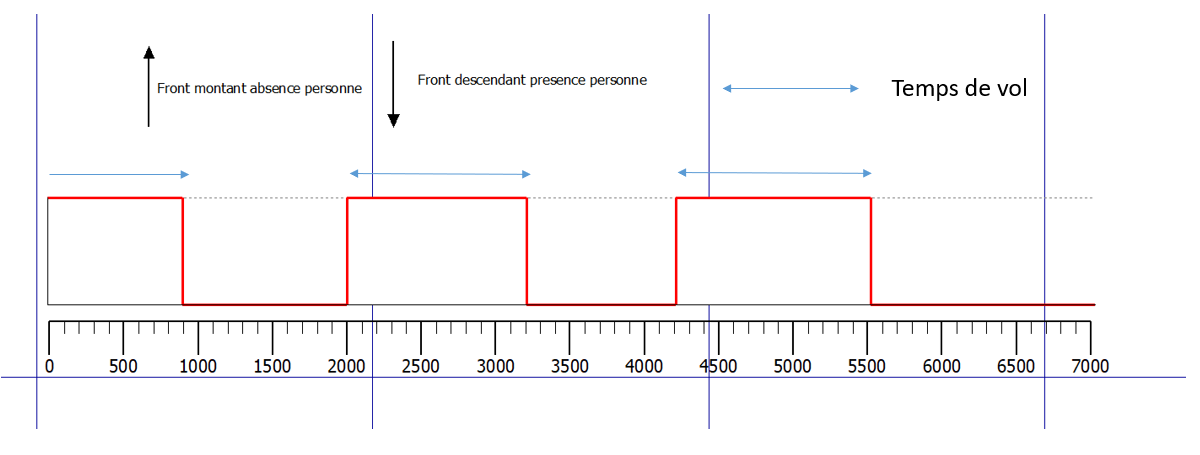
\includegraphics[width=17cm]{photoMohamed/diagramme1ereversion.png}}

Figure 1 – Signal simple

\end{center}

On a ensuite réalisé une autre version du chronomètre qui prenait en compte les rebonds. Notre objectif était d’éliminer les perturbations liées aux rebonds, causés par les vibrations du trampoline. On a ensuite identifié deux types de rebonds. Une première catégorie de rebonds dus aux vibrations causées par la personne présente sur la toile et une deuxième catégorie de rebonds liés aux lasers qui passent entre le maillage de la toile du trampoline. (Voir figure 2 et 3)

\begin{center}
\makebox[\textwidth]{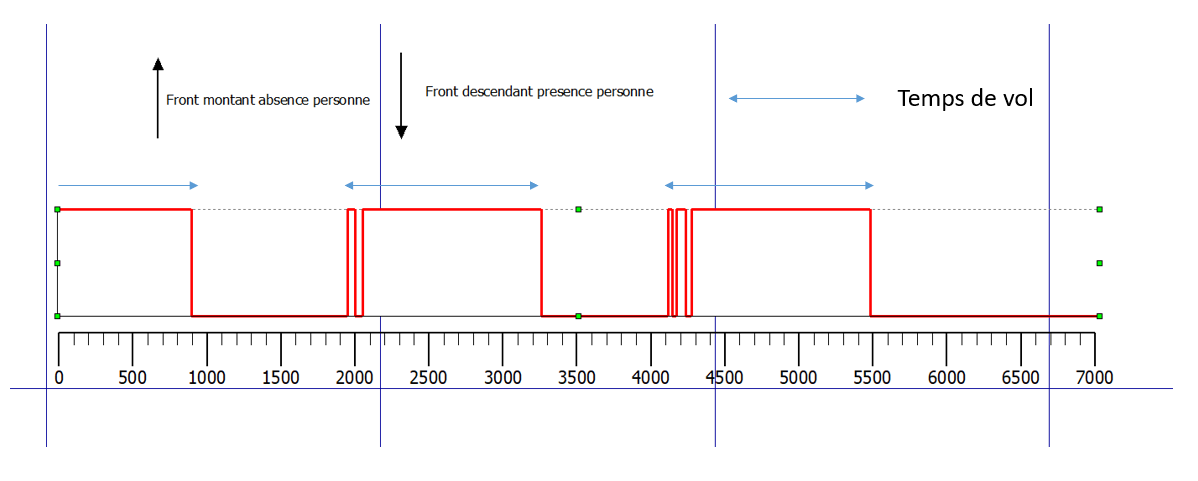
\includegraphics[width=17cm]{photoMohamed/diagramme2.png}}
  
Figure 2 – Signal perturbé par le décollage d’un individu
\end{center}

\begin{center}
\makebox[\textwidth]{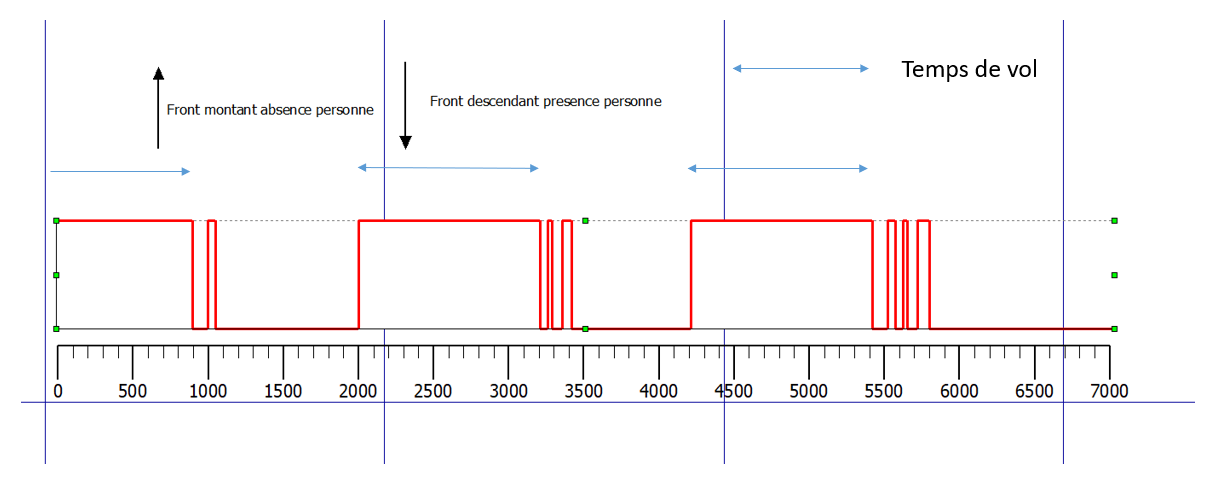
\includegraphics[width=17cm]{photoMohamed/diagramme3.png}}
  
Figure 3 – Signal perturbé par l’atterrissage d’un individu 
\end{center}

Notre solution à ce problème est l’implémentation d’un seuil antirebonds qui prenait en compte le temps minimal de chaque état, et qui refuse n’importe quelle mesure en dessous de ce seuil. Cette solution traite un signal (voir ci-dessus), où l’on élimine chaque état haut qui a une durée inférieure au seuil établi. Après avoir réalisé quelques tests, nous avons choisi un seuil de 300ms. Ce seuil prend en compte qu’une personne reste en l’air au minimum 500 ms. Le seuil est donc suffisamment grand pour éliminer tout type de perturbation, mais suffisamment petit pour prendre en compte les plus petits sauts.

Cependant notre objectif final est d’implémenter un chronomètre qui puisse gérer des perturbations liées aux interférences(perturbation liée à la coupure du faisceaux laser par des éléments externes, indépendamment des fronts). Sachant que lors de nos tests dans le gymnase nous n'avions pas constaté d’interférences, il fallait quand même implémenter cette fonctionnalité car c'est un cas qui pourrait entraîner des erreurs de mesures. Ce seuil prend en compte l’état bas du signal. Si celui-ci est inférieur au seuil, on ne le prend pas en compte et l'on revient au dernier front montant, ce qui nous permet d’éliminer le bruit et d'avoir une mesure plus robuste. (Voir figure 4 ci-dessous).

\begin{center}
    \makebox[\textwidth]{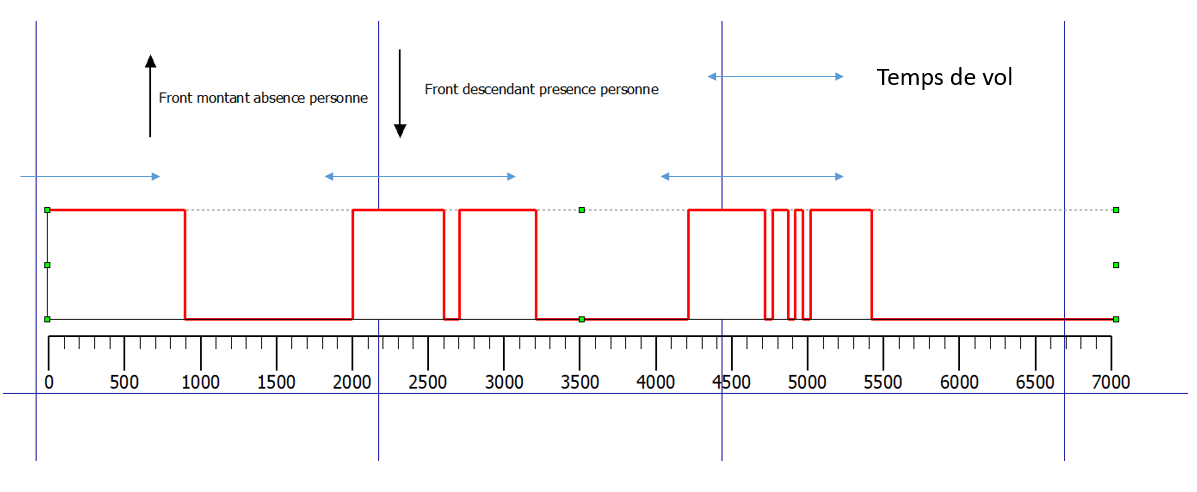
\includegraphics[width=17cm]{photoMohamed/diagramme4.png}}
      
    Figure 4 – Signal bruité par des interférences
\end{center}

Notre programme Chronomètre (ou modeMesure) arrive à transformer un signal bruité, lié à des interférences ou des rebonds et simule un signal sans bruit ou l’on mesure l’état haut à chaque front montant. (Voir exemple figure 5) 

\begin{center}
    \makebox[\textwidth]{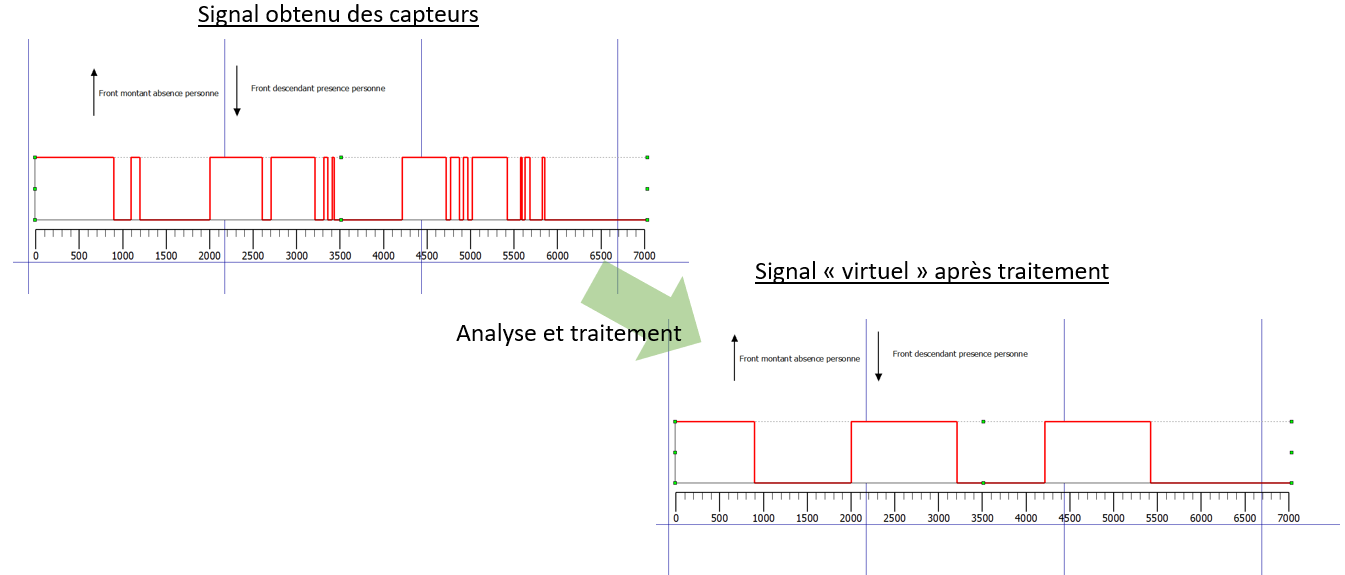
\includegraphics[width=19cm]{photoMohamed/diagramme5.png}}
      
    Figure 5 – Signal avant et après traitement
\end{center}

\subsubsection{Tableau des mesures}
\begin{center}
    \makebox[\textwidth]{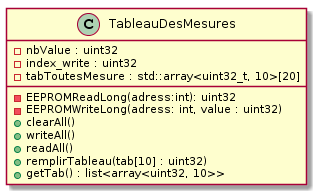
\includegraphics[width=13cm]{photoMohamed/figure6.png}}
      
    Figure 6 – Diagramme UML TableauDesMesures
\end{center}

Cette classe a comme fonction d'écrire et lire dans la mémoire Flash. Nous avons créé cette classe qui utilise comme variable une matrice de 20 tableaux de 10 mesures en entier non signées de 32 bits. L’idée est d’utiliser ce tableau comme intermédiaire pour écrire ou lire dans la mémoire. Donc nos mesures sont enregistrées dans ce tableau, de façon à lire la dernière mesure que l’on a stockée. Ceci est appelé LIFO (Last in, First out). À chaque nouvelle acquisition, les 10 mesures sont stockées dans ce tableau à l'emplacement du curseur (index\_write). On a ensuite développé des fonctions qui permettent d’écrire toute la matrice dans la mémoire, grâce à la librairie Arduino qui nous fournissait ces fonctionnalités. L'écriture se fait par paquet de 8 bits. Nous avons créé notre propre fonction, qui décomposait nos entiers non signés de 32 bits en 4 morceaux d’entiers non signés de 8 bits que nous pouvions ensuite écrire ou lire dans la mémoire Flash.

\begin{center}
    \makebox[\textwidth]{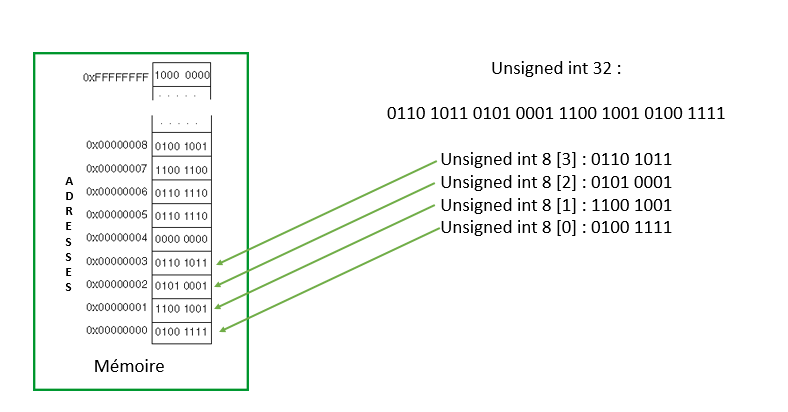
\includegraphics[width=15cm]{photoMohamed/figure7.png}}
      
    Figure 7 – Décomposition de uint32 en uint8
\end{center}

\subsubsection{Site internet}
Le site internet doit afficher les mesures de temps de vol. Pour cela nous avons décidé d'afficher deux formats des données en parallèle : un tableau avec les mesures de chacun des sauts et un graphique prenant le numéro du saut en abscisse et le temps de vol en ordonnée.

Le site internet a été codé en HTML, CSS et JavaScript. En effet, toute la partie affichage de la page est faite du côté client, au travers du navigateur. Le serveur ne fait qu'envoyer le code de la page. Il fallait prendre en compte qu'il n'y a pas d'accès à internet sur le réseau local mis en place par la machine à temps de vol. Cela implique que l'inclusion d'une bibliothèque doit forcément se faire en ajoutant le code source de la bibliothèque au code. Il fallait aussi prendre en compte que la taille de la mémoire flash est de quatre mégaoctets. Malgré ces contraintes nous devions afficher un graphique représentant les mesures. Dans un premier temps, nous avons essayé de trouver une librairie JavaScript suffisamment légère et utilisable à des fins commerciales pour ne pas avoir de restriction en cas d'évolution du projet. Malheureusement, nous n'avons pas réussi à trouver et c'est pour cela qu'il a fallu coder nous-mêmes une librairie d'affichage de graphiques.

Le microcontrôleur a peu de RAM et la gestion de chaîne de caractère très grande est problématique. Le code a donc été fait pour que le JavaScript génère lui-même le code HTML et CSS. Cela permet de déplacer la partie génération du code sur le navigateur du client. Donc nous injectons directement les mesures dans le JavaScript. C'est ce qui est fait dans la classe HTMLgenerator : elle ajoute les mesures en dure dans le code HTML. Pour cela le tableau de mesures est converti en une chaîne de caractère correspondant à la déclaration du tableau en Javastring.

Les mesures sont ensuite traitées par le site pour être affichées. La cliente nous a explicitement demandé de pouvoir récupérer les mesures sur Microsoft Excel. Cette fonctionnalité a demandé beaucoup de recherches, car il ne fallait pas utiliser une bibliothèque trop grande. Finalement une solution très simple a été trouvée en appelant directement l'application Excel depuis le navigateur plutôt que de générer un fichier de sauvegarde standard. Cette solution ne fonctionne que si Excel est installé, mais après plusieurs tests, plusieurs autres applications de tableur sont compatibles avec cette commande, notamment sur mobile. Si vous êtes intéressé, vous pouvez vous reporter à la fonction « fnExcelReport() » dans le document data/testPageWeb.html. Cette fonction est disponible depuis un bouton « Export to Excel » en haut de la page.

Le dernier cas traité est le cas ou il n'y a pas de mesures. Dans cette situation une page blanche avec le message « Il n'y a pas de mesures » est envoyée.

\begin{center}
  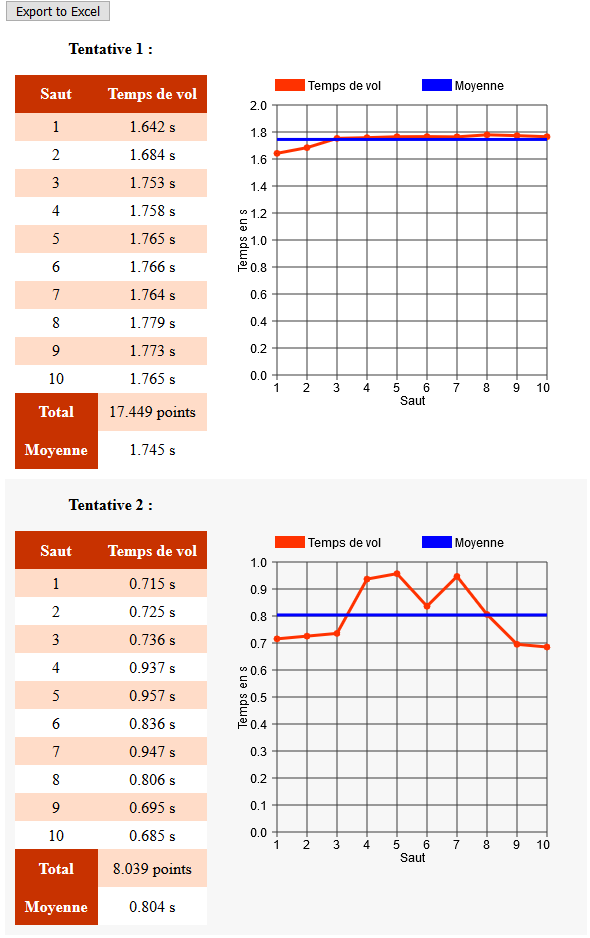
\includegraphics[width=10cm]{photoAlex/siteWEB}
  
  Exemple de deux mesures sur le site internet avec le bouton d'exportation.
\end{center}

\subsubsection{Serveur}
Le serveur a pour but d'afficher le site internet. Il a été codé en C++ à l'aide de plusieurs bibliothèques déjà prévues à cet effet, pour notre "nodeMCU V3" précisément. Le serveur a pour lui 2 bibliothèques : 
\paragraph{ESP8266WebServer.h :}
Elle nous a permis de démarrer et de configurer notre serveur. Incluant des fonctions permettant de définir les modes, les adresses IP, les masques et les différents identifiants et mots de passe, cette bibliothèque nous a permis de générer le serveur en un minimum de lignes de code.
Elle incluait, en plus, des fonctions nous permettant d'afficher nos pages WEB et de générer plusieurs pages en fonction de l'URL rentrée (commençant par notre IP). N'ayant qu'une seule page à afficher, nous l'affichons pour importer l'URL tant qu'il commence par l'IP voulu.
\paragraph{DNSServer.h :}
Celle-là nous a permis d'utiliser un serveur DNS et de rediriger une adresse web vers une autre. Grâce à elle, nous avons pu rediriger l'adresse "www.tempsdevol.com" vers une URL composée de notre adresse IP et cela en seulement 3 lignes.
\paragraph{}
Le serveur a donc été créé et géré grâce à ses 2 bibliothèques. Il a fallu faire beaucoup de recherches pour apprendre à les connaître et utiliser leurs fonctions, mais le serveur a été fait relativement vite par la suite.

\subsubsection{Test}
Chaque classe de notre programme a été faite séparément en utilisant des données simulées et le diagramme de classe fait au début du projet. Les lasers mettant longtemps à arriver, nous avons commencé par tester nos programmes avec de simples boutons. Nous avons d'abord simulé nos lasers avec ses boutons pour tester notre chronomètre puis l'avons ensuite testé avec les vrais lasers. Nous avons alors remarqué quelques rebonds dans les signaux renvoyé capteurs lasers qui nous affichaient de fausses mesures. Il a alors fallu simuler les rebonds informatiquement et modifier le chronomètre pour qu'il ne soit plus affecte par eux. Une fois la programmation de nos parties respectives terminée, nous avons commencé à les intégrer dans un ordre prédéfini afin de diminuer les erreurs qui risquaient d’apparaître par la suite. L’ordre des intégrations était : Réseau$\,\to\,$PageWeb$\,\to\,$chronomètre/temps de vol$\,\to\,$écran$\,\to\,$programme principal. Le but de chacune de ces intégrations était :
\paragraph{Réseau :}
Nous avons commencé par vérifier que notre serveur est capable d’afficher une page internet correctement.
\paragraph{PageWeb :}
Le but de cette première intégration était alors de générer des pages web différentes avec des données simulées, puis de vérifier que le réseau actualise bien la page web affichée. 
\paragraph{Chronomètre/temps de vol :}
Le but de cette partie étant de mesurer une donnée extérieure, nous avons fixé les lasers utilisés de façon à simuler l’utilisation du chronomètre sur le trampoline. Il fallait alors retourner les mesures de chronomètre pour générer la nouvelle page web puis l’afficher sur le réseau.
\paragraph{Écran :}
Il fallait alors retourner les mesures de chaque saut et le temps total vers l’écran pour nous permettre d’utiliser la machine à temps de vol sans avoir un appareil avec une connexion au réseau.
\paragraph{Programme principal :}
Pour finir, il fallait alors intégrer les 3 lasers dans le programme (nous n’en utilisions qu’un seul jusqu’à maintenant) et de rajouter une LED indiquant si oui ou non les lasers sont coupés (ou s’ils ne sont pas bien mis en place)

%programme principale
\subsubsection{Programme principal}
Le programme principal est assez simple puisque toutes les fonctionnalités les plus importantes ont été déportées dans les classes. Le programme principal gère la lecture des entrées et l'allumage de la LED au travers d'interruptions et à l'aide des différentes classes créées. Le diagramme qui suit est le diagramme de classe final. Il est plus grand que le diagramme initial et montre bien l'évolution du projet entre la conceptualisation et la conception.

\begin{center}
  \makebox[\textwidth]{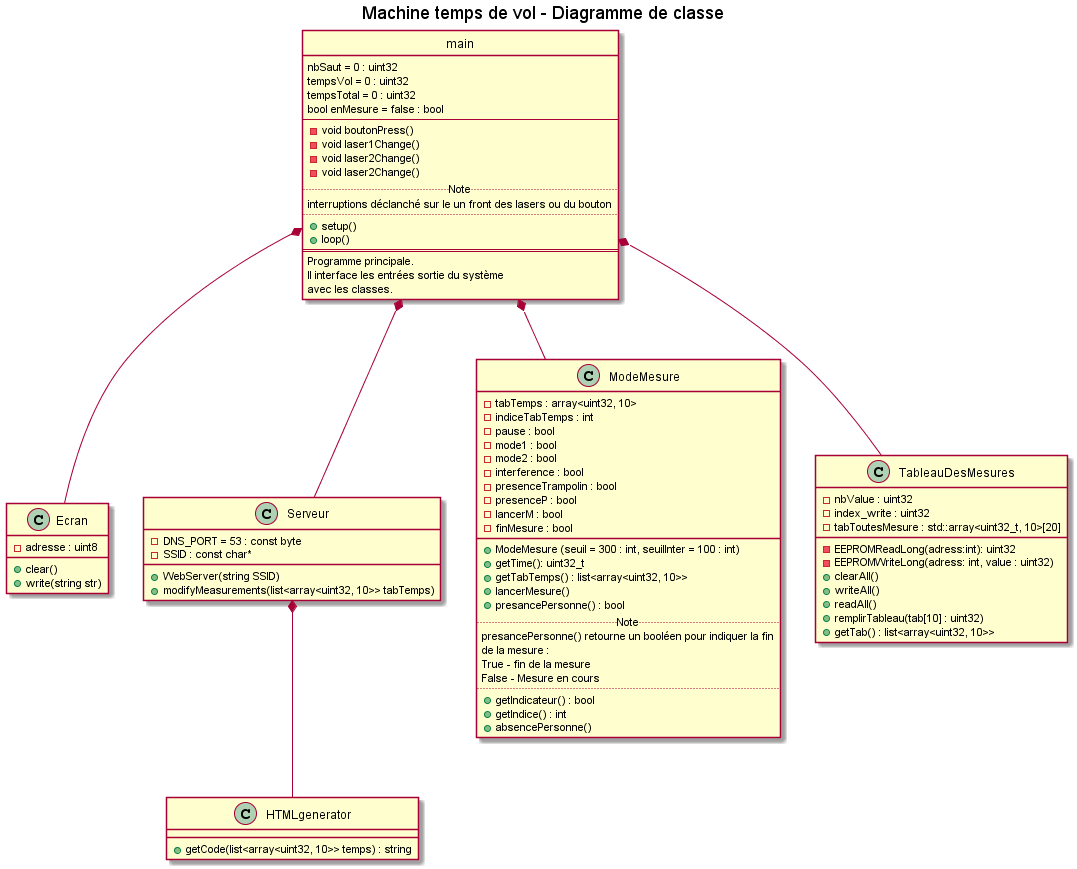
\includegraphics[width=19cm]{photoAlex/diagrammeDeClasse.png}}
  
  Diagramme de classe final
\end{center}

%Réseau
\subsection{Réseau}
Le composant que nous avons choisi d’utiliser, le « nodeMCU V3 », a l’avantage d’intégrer directement un module WIFI et le réseau a pu être intégré grâce à lui. Ce module reste tout de même une partie à part du composant. Pour l’utiliser, il fallait tout d’abord flasher la carte pour paramétrer le module Wifi et y assigner toutes les données dont il fallait disposer pour l’utiliser, telles que les adresses MAC.
\begin{center}
    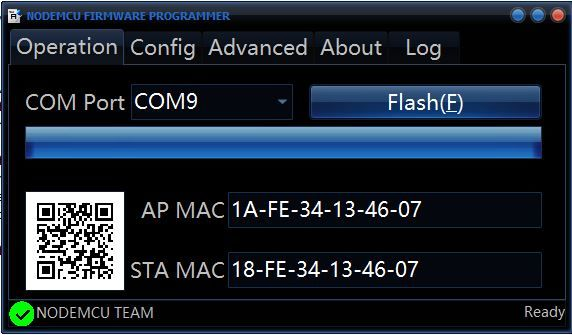
\includegraphics[scale=0.4]{photoHugo/image001}
    
    Flash du module WIFI
\end{center}
Une fois fait, les paramètres étaient gardés en mémoire et il s’agissait alors de définir les paramètres de notre serveur pour utiliser le réseau comme nous le voulions : le mode, l’adresse IP, le masque, l’identifiant et le mot de passe. Le module WIFI a à disposition 2 modes : le mode point d’accès (AP) et le mode relais (STA) permettant de relayer un réseau existant. Les modes étant initialement tout les deux activés, nous commençons donc par forcer l’activation du mode AP uniquement. L’adresse IP a été fixée à 192.168.4.1 et le masque à 255.255.255.0 permettant ainsi à 254 hôtes de se connecter au réseau (en supposant que notre composant le supporte). L’identifiant du réseau est « tempsDeVol » afin d’être facilement reconnaissable, nous ne divulguerons cependant pas le mot de passe qui a seulement été donné à notre cliente. N’ayant qu’une page internet à afficher, celle-ci s’affiche automatiquement lorsque l’on tape l’adresse IP dans la barre de recherche.
\begin{center}
    \makebox[\textwidth]{
        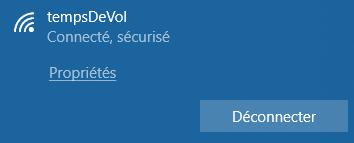
\includegraphics[width=0.6\textwidth]{photoHugo/Capture3}
        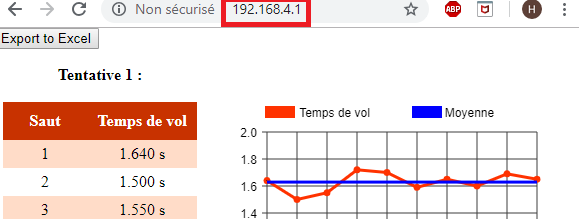
\includegraphics[width=0.6\textwidth]{photoHugo/Capture2}
        }
    
    Connection à la page web
\end{center}

\normalsize
Pour faciliter la recherche, nous utilisons un serveur DNS pour rediriger une autre adresse internet simple à retenir vers notre adresse IP. Nous avons donc choisi de rediriger l’adresse « www.tempsdevol.com » pour y retrouver nos mesures.

\begin{center}
    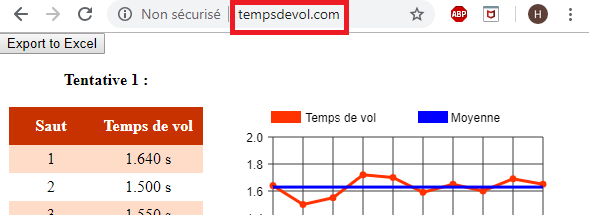
\includegraphics[width=0.9\textwidth]{photoHugo/Capture1}

    Redirection de l'adresse "www.tempsdevol.com"
\end{center}

\normalsize
%Conception des boîtiers et supports
\subsection{Boîtiers et supports}
\subsubsection{Supports récepteurs}
Au vu des avancées de l’équipe sur les programmes gérant la page internet, le réseau et la mesure du temps de vol, il a été rapidement nécessaire de pouvoir mettre le programme de mesure du temps de vol à l’épreuve des conditions réelles. Nous ne savions alors pas vraiment comment le trampoline allait se comporter durant un exercice en condition de compétition, mais nous savions qu’il pourrait avoir un impact sur les performances du programme de mesure. Il était nécessaire d’imaginer les scénarios pouvant poser des problèmes : que se passe t-il si on ne finit pas la série de dix sauts ? Que se passe t-il si un athlète reste sur la toile ? L’effet de tous ces cas non conformes à une utilisation standard ont nécessité un prototype pour pouvoir être finement appréhendés. De plus, nous devions, à terme, mettre au point un dispositif robuste aux oscillations mécaniques, autrement dit, aux vibrations, et nous voulions pouvoir expérimenter des prototypes au plus vite.

Le premier prototype est une simple boîte, permettant d’y loger un pointeur LASER, ou un récepteur. Cette boîte était faite pour être assemblée grâce à des accessoires facilement trouvables en boutique de bricolage : un jeu de 4 vis et un autre de 4 aimants. Ce prototype nous a principalement permis de comprendre qu’une aimantation assez forte contre le cadre horizontal du trampoline serait suffisante pour avoir un système convenablement stable. Il a également permis à l’équipe développant le programme de mesure de comprendre , qu’il était obligatoire de considérer des problèmes dit de rebond; phénomène d'oscillations non contrôlés pouvant être observés sur un signal électrique, parfois dus au dispositif générant le signal, ici, les récepteurs LASER, et parfois dû à l’équipement sujet à la mesure, ici notamment, l’aspect maillé de la toile du trampoline.

\begin{center}
  \makebox[\textwidth]{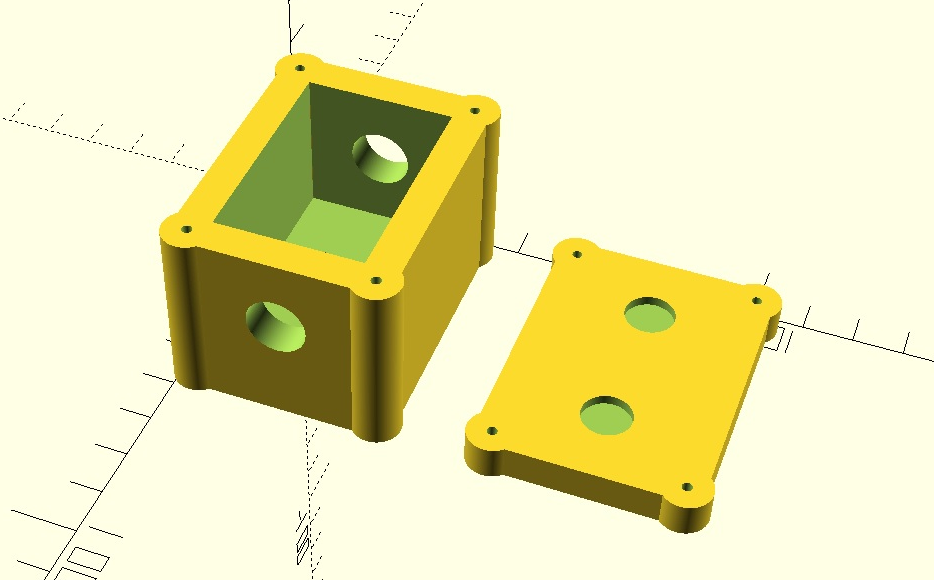
\includegraphics[width=8cm]{photoFrancois/image1}}
  
  Prototype initial
\end{center}

Il a permis aussi de voir émerger l’idée de positionner les capteurs et les récepteurs sur la largeur du trampoline, et non plus sur la longueur, afin de les rapprocher, la distance ayant un impact direct sur l’observation de l’amplitude de l'oscillation d’un point projeté.

\begin{center}
  \makebox[\textwidth]{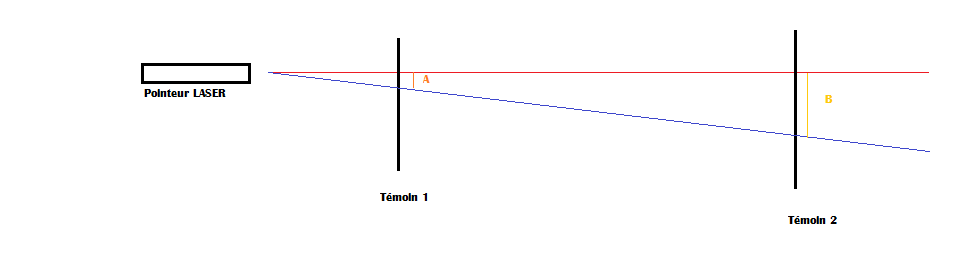
\includegraphics[width=15cm]{photoFrancois/image2}}
  
  Trajectoire du laser
\end{center}

Le prototype final prend en compte tous les aspects déjà évoqués, il permet principalement d’être conforme au nouveau support pour l'émetteur, qui se devait d’être plus facilement réglable. Le support de l'émetteur sera décrit plus en avant dans ce document.

\begin{center}
  \makebox[\textwidth]{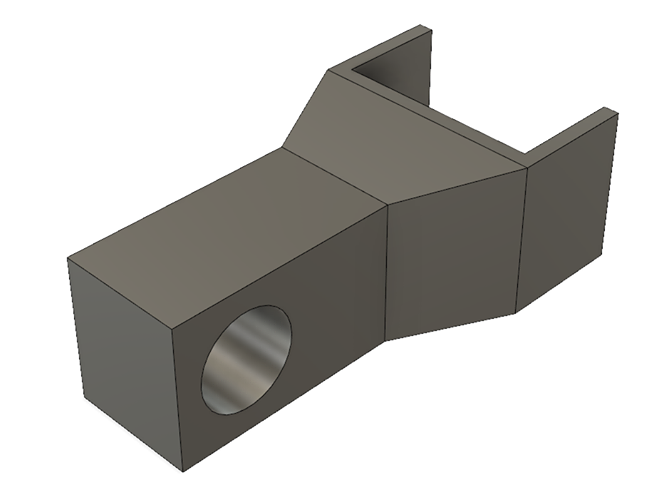
\includegraphics[width=8cm]{photoFrancois/image3}}
  
  Prototype final du récepteur
\end{center}

\subsubsection{Supports laser}
Les supports des lasers (émetteur et récepteur) sont tout deux partis du boîtier les lasers récepteurs que nous avons graduellement améliorés pour corriger deux problèmes : la fixation du laser contre le trampoline et la modification de la hauteur du laser pour qu’il atteigne le récepteur. Toujours à l’aide d’imprimante 3D, nous sommes partis du boîtier de base et avons pensé à plusieurs prototypes :

\paragraph{Prototype n°1 :}
Le but était de lever ou baisser l’arrière du laser pour en modifier la hauteur. Ce n'était pas assez fiable et il n'y avait pas assez de marge de manœuvre.
\begin{center}
    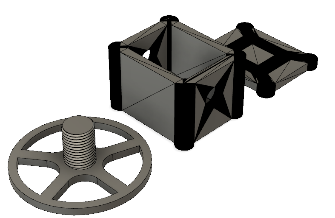
\includegraphics{photoHugo/image005}
    
    Prototype n°1 
\end{center}

\paragraph{Prototype n°2 :}
Un système mécanique entièrement imprimé en 3D : il se serait vite abîmé et n’aurait pas eu une bonne durée de vie.
\begin{center}
    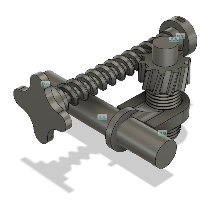
\includegraphics{photoHugo/image007}
    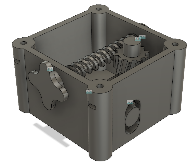
\includegraphics{photoHugo/image009}
    
    Prototype n°2
\end{center}

\paragraph{Prototype n°3 :}
Une meilleure mise en place des aimants et une modification de la hauteur du laser fait par de vrais vis et écrous. Une meilleure durée de vie, mais l'on remarque que les aimants ne sont pas assez puissants lorsque des adultes sautent.
\begin{center}
    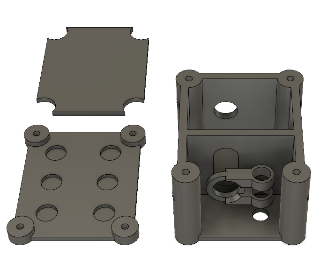
\includegraphics{photoHugo/image011}
    
    Prototype n°3
\end{center}

\paragraph{Prototype n°4 :}
Ajout de nouveaux aimants plus puissants sur les côtés du boîtier. Le système est fonctionnel, mais la forme de boite n’étant plus utile pour poser les aimants sur le couvercle, on revoit toute la structure.
\begin{center}
    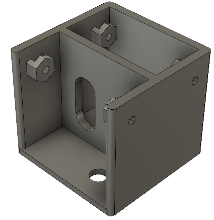
\includegraphics{photoHugo/image013}
    
    Prototype n°4
\end{center}

\paragraph{Prototype n°5 :}
Nous partons alors sur un système beaucoup plus minimaliste ou l’on utilise une vis pour modifier l’inclinaison du laser et l'on visse un écrou pour fixer la position du laser : le système est utilisable, mais il y a un petit jeu sur les aimants et l’on doit forcer sur l’écrou (même avec une aide) pour que le laser ne bouge plus.
\begin{center}
    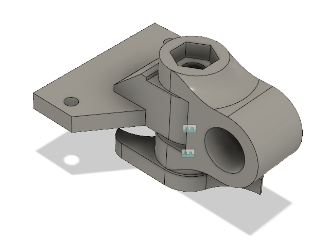
\includegraphics{photoHugo/image015.png}
    
    Prototype n°5
\end{center}

\paragraph{Prototype n°6 :}
Nous réglons les 2 derniers problèmes, une vis de serrage rapide est ajoutée pour faciliter la fixation du laser et les aimants sont enlevés de leurs supports de base et fixés manuellement : le prototype est entièrement fonctionnel. 
\begin{center}
    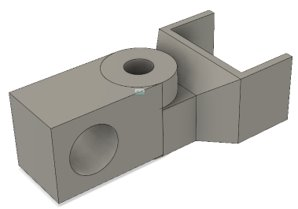
\includegraphics[width=0.4\textwidth]{photoHugo/image017}
    
    Prototype n°6
\end{center}

Nous arrivons finalement à un prototype entièrement fonctionnel et économe en quantité de plastique et de temps d’impression. Après avoir fini de prototyper la fixation de nos lasers émetteurs, nous avons refait la fixation du laser récepteur de la même façon. Même si le prototype actuel est fonctionnel, nous pourrions encore l'améliorer à l'avenir. 
\begin{center}
    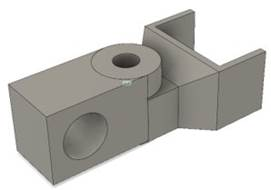
\includegraphics[width=0.4\textwidth]{photoHugo/image019}
    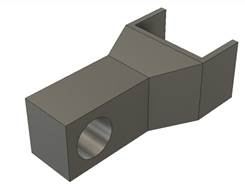
\includegraphics[width=0.4\textwidth]{photoHugo/image021}
    
    Prototype final (laser émetteur et récepteur)
\end{center}

\subsubsection{Boîtiers}
En plus de la fixation des lasers, nous avons imprimé plusieurs boîtiers afin d’y fixer les connectiques de nos lasers, les alimentations et de protéger l’utilisateur des soudures. Nous avons alors eu deux boîtiers à imprimer :
\paragraph{Le boîtier d’alimentation}
Il a pour but d’alimenter les 3 lasers émetteurs présents du côté opposé à celui où va se trouver l’utilisateur de la machine à temps de vol. Il prend en entrée 1 jack d’alimentation (le câble étant fourni) et en sortie les 3 jacks des 3 lasers émetteurs.
\begin{center}
    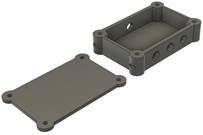
\includegraphics[width=0.4\textwidth]{photoHugo/image023}
    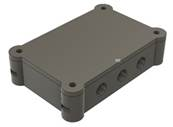
\includegraphics[width=0.4\textwidth]{photoHugo/image025}
    
    Boîtier d'alimentation
\end{center}
\paragraph{Le boîtier de contrôle}
Il s’agit du boîtier que l’utilisateur va avoir en main. Il inclut les 3 jacks des 3 lasers récepteurs, 1 jack pour l’alimentation et un accès aux interfaces présents sur le composant (écran, bouton et LED). 
\begin{center}
    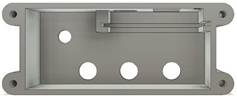
\includegraphics[width=0.4\textwidth]{photoHugo/image027}
    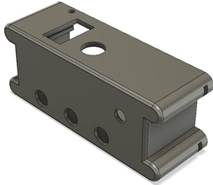
\includegraphics[width=0.4\textwidth]{photoHugo/image029}
    
    Boîtier de contrôle
\end{center}

%Câblage
\subsection{Câblage}
Le schéma qui suit est le câblage qui a été fait sur le prototype. La grille représente la carte PCB de prototypage qui est prépercée suivant cette grille. Les ronds blancs représentent les séparations entre les composants et les carrés sont les pins du microcontrolleur, de l'écran, ou des capteurs.
\begin{center}
    \makebox[\textwidth]{\begin{circuitikz}[european,scale=0.85]

%generation de la grille
\newcounter{ct}

\forloop{ct}{0}{\value{ct} < 15}
{
  \draw[dashed] (-0.5 + \value{ct}, -0.5) -> (-0.5 + \value{ct}, -0.5 + 20);
}

\forloop{ct}{0}{\value{ct} < 21}
{
  \draw[dashed] (-0.5, -0.5 + \value{ct}) -- (-0.5 + 14,-0.5 + \value{ct});
}

\forloop{ct}{1}{\value{ct} < 15}
{
  \node at (\value{ct}-1,20){\arabic{ct}};
}

\forloop{ct}{1}{\value{ct} < 21}
{
  \node at (14,21 - \value{ct}-1){\Alph{ct}};
}

%nodeMCU
\node[draw] (D0) at (1,15) {$D0$};
\node[draw] (D1) at (1,14) {$D1$};
\node[draw] (D2) at (1,13) {$D2$};
\node[draw] (D3) at (1,12) {$D3$};
\node[draw] (D4) at (1,11) {$D4$};
\node[draw] (3V1) at (1,10) {$3V$};
\node[draw] (G1) at (1,9) {$G$};
\node[draw] (D5) at (1,8) {$D5$};
\node[draw] (D6) at (1,7) {$D6$};
\node[draw] (D7) at (1,6) {$D7$};
\node[draw] (D8) at (1,5) {$D8$};
\node[draw] (RX) at (1,4) {$RX$};
\node[draw] (TX) at (1,3) {$TX$};
\node[draw] (G2) at (1,2) {$G$};
\node[draw] (3V2) at (1,1) {$3V$};

\node[draw] (A0) at (12,15){$A0$};
\node[draw] (G3) at (12,14) {$G$};
\node[draw] (VU) at (12,13) {$VU$};
\node[draw] (S3) at (12,12) {$S3$};
\node[draw] (S2) at (12,11) {$S2$};
\node[draw] (S1) at (12,10) {$S1$};
\node[draw] (SC) at (12,9) {$SC$};
\node[draw] (S0) at (12,8) {$S0$};
\node[draw] (SK) at (12,7) {$SK$};
\node[draw] (G4) at (12,6) {$G$};
\node[draw] (3v3) at (12,5) {$3V$};
\node[draw] (EN) at (12,4) {$EN$};
\node[draw, scale=0.8] (RST) at (12,3) {$RST$};
\node[draw] (G5) at (12,2) {$G$};
\node[draw, scale=0.8] (VIN) at (12,1) {$VIN$};

%PIN ecran
\node[draw, scale=0.8] (VCC) at (5,18) {$VCC$};
\node[draw, scale=0.75] (GND) at (6,18) {$GND$};
\node[draw, scale=0.8] (SCL) at (7,18) {$SCL$};
\node[draw, scale=0.8] (SDA) at (8,18) {$SDA$};

%LED
\draw (D0.north) -- (1,19) to[short,-o] (13,19) to[short,-o, empty led] (13,18) to[short,-o] (13,17) to[R={\parbox{1cm}{\SI{100}{\ohm}}}] (13,14) to[short,o-] (G3.east);

%Bouton (bas)
\draw (3V2.east) to[short,-o] (2,1) to[R={\parbox{1cm}{\SI{1000}{\ohm}}}] (6,1) to[short,o-] (6,2);

%Bouton (haut)
\draw[brown] (6,7) to[short] (6,8) to[short] (D5.east);
\draw (4,7) to[short] (4,9) to[short] (G1.east);

%Bouton
\draw
    (6,2) to[short,o-o] (6,7)
    (4,4.5) to[push button] (6,4.5)
    (4,2) to[short,o-o] (4,7)
;
\node[text width=3cm] at (6,5.8){Bouton};

%ecran
\draw[red] (VU.west) to[short] (9,13) to[short] (9,16) to[short] (5,16) to[short] (VCC.south);
\draw (G3.west) to[short] (10,14) to[short] (10,17) to[short] (6,17) to[short] (GND.south);
\draw[blue] (D1.east) to[short] (8,14) to[short] (SDA.south);
\draw[green] (D2.east) to[short] (7,13) to[short] (SCL.south);
\node[text width=3cm] at (6.2,18.8){Ecran};

%alim
\draw[red] (12, -1) to[short, o-] (12,0) to[short] (13,0) to[short] (13,13) to[short] (VU.east);
\draw (10, -1) to[short, o-] (10,2) to[short] (G5.west);

\draw (10, -1) to[V=5V] (12, -1);

%capteur 1
\node[draw, scale=0.8] (C1O) at (-2,12){$OUT$};
\draw (C1O.east) to[R={\parbox{1cm}{\SI{1000}{\ohm}}}] (0,12) to[short, o-] (D3.west);
\node[draw, scale=0.8] (C1G) at (-3,12) {$GND$};
\node[draw, scale=0.8] (C1V) at (-4,12) {$VCC$};
\node[text width=3cm] at (-4.5,12.5){Capteur 1};

%capteur 2
\node[draw, scale=0.8] (C2O) at (-2,7){$OUT$};
\draw (C2O.east) to[R={\parbox{1cm}{\SI{1000}{\ohm}}}] (0,7) to[short, o-] (D6.west);
\node[draw, scale=0.8] (C2G) at (-3,7) {$GND$};
\node[draw, scale=0.8] (C2V) at (-4,7) {$VCC$};
\node[text width=3cm] at (-4.5,7.5){Capteur 2};

%capteur 3
\node[draw, scale=0.8] (C3O) at (-2,6){$OUT$};
\draw (C3O.east) to[R={\parbox{1cm}{\SI{1000}{\ohm}}}] (0,6) to[short, o-] (D7.west);
\node[draw, scale=0.8] (C3G) at (-3,6) {$GND$};
\node[draw, scale=0.8] (C3V) at (-4,6) {$VCC$};
\node[text width=3cm] at (-4.5,6.5){Capteur 3};

\draw 
    (C1G.south) -- (C2G.north)
    (C2G.south) -- (C3G.north) 
    (C3G.south) -- (-3,-1) -- (10, -1)
    ;
    
\draw[red]
    (C1V.south) -- (C2V.north)
    (C2V.south) -- (C3V.north) 
    (C3V.south) -- (-4,-2) -- (12, -2) -- (12, -1)
    ;

\end{circuitikz}
}
\end{center}

\subsection{La conception de la video}
La vidéo avait pour but de présenter rapidement le contexte de notre travail et ce que nous avions réalisé. Nous voulions un plan avec la cliente expliquant son idée et ce pour quoi elle avait fait appel à l’Upssitech. Le montage des différents plans s’est fait à l’aide du logiciel AfterEffect, un logiciel de montage semi-professionnel très souvent utilisé par les monteurs intervenant sur des vidéos diffusées sur internet. L’idée était de faire se succéder différents plans structurants sans trop détailler le cheminement du travail que nous avions réalisé, jusqu'à la démonstration finale, présentant sous différent points de vus synchronisés, le comportement du produit en situation réelle. La musique choisie est libre de droit, Up \& Away de JPB.

\begin{center}
  \makebox[\textwidth]{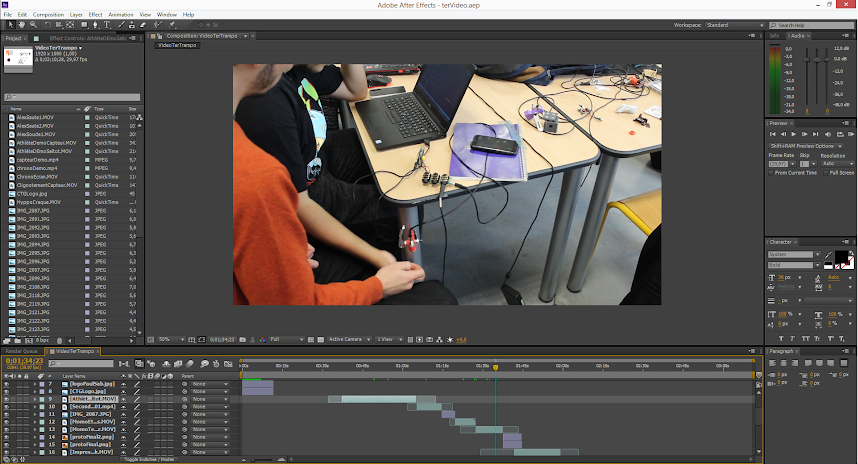
\includegraphics[width=18cm]{photoFrancois/image4}}
  $www.youtube.com/watch?v=wKbeXyNoAr4$
\end{center}
